\section{11. Evaluation and results}

\subsection{11.1 Setup}

Four policies were run over the same simulated week, after a training week
that the predictor learned from. Every table in this section is generated by
\code{cmd/evaluate} from the stored records of the runs named here.

\begin{longtable}[]{@{}L{0.16\linewidth}L{0.76\linewidth}@{}}
\toprule
\endhead
\textbf{Building} & 50 rooms on the ground floor: 3 fika rooms, 20 lecture rooms, 24 offices and 3 unused rooms; 5 devices each \\
\textbf{Training} & Run \code{train-week-v2}: reactive policy, Mon 14 to Fri 18 Sep 2026, factor 120; 360\,000 people-counter readings; model \code{profile-train-week-v3} \\
\textbf{Evaluation} & Mon 21 to Fri 25 Sep 2026, held out from training, factor 120. Runs \code{eval-constant-v2}, \code{eval-reactive-v2}, \code{eval-predictive-v3} and \code{eval-oracle-v2}, which replays the true occupancy of \code{eval-reactive-v2} \\
\textbf{Fairness} & Same rooms, devices and dates; physics starts every run from fresh rooms; only the policy differs. Verified: all four runs have the same head-count and guard count in every one of 360\,500 shared truth records \\
\textbf{Heating} & The same in every run: schedule with optimal start \\
\textbf{Occupied} & A room counts as occupied when someone other than a guard on patrol is in it. The 481 guard-only records per run are counted separately \\
\textbf{Data} & One truth record per room and model minute, 7\,211 minutes, about 2.16 million records per run, none rejected by storage. At least 99.9~\% of sensor readings of every kind arrived \\
\bottomrule
\end{longtable}

\subsection{11.2 Air quality, comfort and energy}

\begin{longtable}[]{@{}L{0.36\linewidth}L{0.13\linewidth}L{0.13\linewidth}L{0.13\linewidth}L{0.13\linewidth}@{}}
\toprule
 & \textbf{Constant} & \textbf{Reactive} & \textbf{Predictive} & \textbf{Oracle} \\
\midrule
\endhead
\COtwo{} at or below 1000 ppm, occupied (NFR-1: at least 95~\%) & 95.5~\% & 100.0~\% & 100.0~\% & 100.0~\% \\
\quad in lecture rooms only & 65.2~\% & 100.0~\% & 100.0~\% & 100.0~\% \\
Occupied room-minutes above 1000 ppm & 612 & 4 & 0 & 0 \\
Peak \COtwo{} & 1084 ppm & 1024 ppm & 972 ppm & 968 ppm \\
20--24 °C, occupied (NFR-2: at least 95~\%) & 100.0~\% & 100.0~\% & 100.0~\% & 100.0~\% \\
Energy over the week & 25\,285 kWh & 6\,282 kWh & 6\,521 kWh & 6\,370 kWh \\
Saving against constant (NFR-3: at least 30~\%) & & 75~\% & 74~\% & 75~\% \\
Energy against reactive & +302~\% & & +3.8~\% & +1.4~\% \\
\bottomrule
\end{longtable}

\begin{figure}[H]
\centering
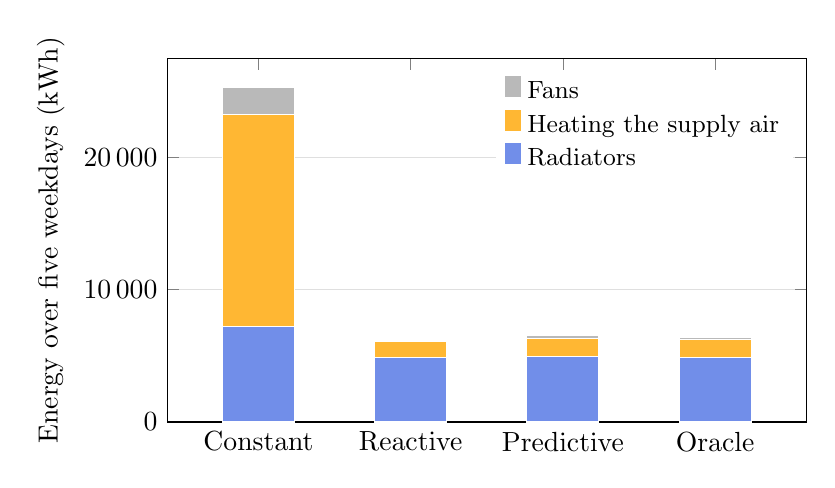
\begin{tikzpicture}
\begin{axis}[
  ybar stacked, width=0.80\linewidth, height=6.2cm, bar width=26pt,
  ymin=0, ymax=27500, enlarge x limits=0.2,
  ylabel={Energy over five weekdays (kWh)},
  symbolic x coords={Constant,Reactive,Predictive,Oracle}, xtick=data,
  scaled y ticks=false, yticklabel style={/pgf/number format/fixed,/pgf/number format/1000 sep={\,}},
  ymajorgrids, grid style={gray!25},
  legend style={at={(0.98,0.97)},anchor=north east,draw=none,font=\small},
  legend cell align=left, reverse legend]
\addplot+[fill=RoyalBlue!75,draw=white] coordinates {(Constant,7224) (Reactive,4892) (Predictive,4933) (Oracle,4908)};
\addplot+[fill=Orange!80,draw=white] coordinates {(Constant,16055) (Reactive,1235) (Predictive,1412) (Oracle,1300)};
\addplot+[fill=gray!55,draw=white] coordinates {(Constant,2007) (Reactive,154) (Predictive,176) (Oracle,162)};
\legend{Radiators,Heating the supply air,Fans}
\end{axis}
\end{tikzpicture}
\caption{The energy proxy by part. Almost all of the difference between
constant flow and the other policies is the heating of supply air that nobody
needed. The three demand-controlled policies differ by a few per cent.}
\label{fig:energy}
\end{figure}

\textbf{Constant ventilation is expensive and still not good enough.} Design
flow day and night costs four times the energy of the other policies, and full
lecture rooms still exceed 1000~ppm in a third of their occupied minutes. That
is what the sizing table in Section 6 predicts: a full room at design flow
settles right around the limit.

\textbf{Reactive control already does almost all of it.} It meets NFR-1 with
four minutes above 1000~ppm all week, in fika rooms, at the lowest energy.

\textbf{Anticipation buys a little, for a little.} With perfect knowledge of
the future, the oracle removes those four minutes and lowers the peak from
1024 to 968~ppm, for 1.4~\% more energy. Because the four runs saw exactly the
same week, that 1.4~\% is a real difference and not noise. The proposal said
that a small gap between reactive control and the oracle would be a result
worth reporting; here it is. The likely reasons are in the design, not the
policy: a damper reaches 1.5 times design flow within a few minutes, and a
lecture room at design flow has a time constant of 12 minutes, so a reactive
controller catches up fast.

\textbf{The predictor gets the oracle's air quality for 3.8~\% more energy
than reactive.} No occupied minute above 1000~ppm, peak 972~ppm. The 2.4~\% it
spends beyond the oracle is the price of an imperfect forecast: it ventilates
fika rooms for a break on days when the break turns out small, and it reacts
to the counter's occasional false ``one person''. This is where the second
half of NFR-3 fails: \code{predictive} was required to use no more energy than
\code{reactive}, and it uses 3.8~\% more. With these rooms and dampers the
honest conclusion is that reactive control is the better trade unless the last
four minutes above the limit matter.

\textbf{Comfort is met everywhere}, now that heating starts before 07:00.

\missingfigure{Response over time: measured \COtwo{}, people counted and
airflow in fika room 1570 on one morning of the evaluation week, 09:00 to
11:00, for \code{reactive}, \code{predictive} and \code{oracle}. The data is in
the storage volume on the PC that ran the evaluation: storage's
\code{/history} with \code{run=eval-predictive-v3}, \code{room=level0/1570}
and \code, and the same for the other two runs.}

\subsection{11.3 The forecast}

Model \code{profile-train-week-v3} on the held-out run \code{eval-reactive-v2},
at every people-counter reading on weekdays 07--18: the peak count within the
next 20 minutes, against the forecast and against ``same as now''. An arrival
is a rise of at least 5 people within the 20 minutes.

\begin{longtable}[]{@{}L{0.10\linewidth}L{0.11\linewidth}L{0.12\linewidth}L{0.14\linewidth}L{0.10\linewidth}L{0.10\linewidth}L{0.11\linewidth}@{}}
\toprule
\textbf{Role} & \textbf{Readings} & \textbf{Forecast MAE} & \textbf{``Same as now'' MAE} & \textbf{Arrivals} & \textbf{Foreseen} & \textbf{False alarms} \\
\midrule
\endhead
Fika & 9\,900 & 4.23 & 2.33 & 1\,042 & 86.7~\% & 22.6~\% \\
Lecture & 65\,920 & 1.13 & 0.81 & 283 & 0.0~\% & 1.1~\% \\
Office & 79\,122 & 0.60 & 0.64 & 0 & & 0.0~\% \\
\bottomrule
\end{longtable}

\textbf{FR-4 is not met as we wrote it.} The requirement asked for a lower
error than ``same as now'', and by mean absolute error the forecast is worse
in fika and lecture rooms. The measure was badly chosen: the forecast is a high
quantile on purpose, so it overshoots most of the time by design, and ``same as
now'' is right whenever nothing changes, which is most minutes. What the
controller needs from a forecast is warning of an arrival, and there the
picture is the opposite: the forecast foresees 87~\% of the arrivals in fika
rooms, with a false alarm in 23~\% of quiet moments, and ``same as now''
foresees none by definition.

\textbf{It warns ahead of fika breaks, but not of lectures.} In lecture rooms
the forecast foresaw none of 283 arrivals. occupancysim puts each lecture in a
random room every slot and day, so a single room has no pattern to learn, and
no model trained on that room's history could do better. A timetable as an
input would fix it.

\textbf{More data made the model worse.} The first model trained on a reading
per minute expected at least one person in about 86~\% of all 15-minute slots
in every room, nights included, and the predictive run that used it spent
25~\% more energy than reactive, most of it on empty rooms. The cause was how
the training treated the counter's noise. The counter shows one person too many
in about 5~\% of readings. The training took the \emph{highest} reading of each
slot and day, and with 15 readings per slot an empty room shows a false ``1''
on more than half of the days ($1 - 0.95^{15} = 54~\%$). The earlier, thinner
training data had three readings per slot, and the same flaw touched about
15~\% of slots without being noticed. The predictor's unit tests used
noise-free data and passed.

\begin{longtable}[]{@{}L{0.40\linewidth}L{0.13\linewidth}L{0.11\linewidth}L{0.10\linewidth}L{0.10\linewidth}@{}}
\toprule
 & \textbf{Before the fix} & \textbf{After} & \textbf{Reactive} & \textbf{Oracle} \\
\midrule
\endhead
Slots at night in which the model expects someone & 82--88~\% & 0~\% & & \\
Mean airflow in empty rooms at night & 30.9 l/s & 8.7 l/s & 7.5 l/s & 7.7 l/s \\
Mean airflow in empty rooms, 09--17 & 35.1 l/s & 28.3 l/s & 25.8 l/s & 26.6 l/s \\
Energy over the week & 7\,877 kWh & 6\,521 kWh & 6\,282 kWh & 6\,370 kWh \\
Energy against reactive & +25~\% & +3.8~\% & & +1.4~\% \\
Fika arrivals foreseen / false alarms & 97 / 25~\% & 87 / 23~\% & & \\
\bottomrule
\end{longtable}

The fix takes the 75th percentile of a slot's readings and counts a forecast
below half a person as an empty room. The model was retrained on the same
stored week and only the predictive run repeated
(\code{eval-predictive-v2} is kept as the evidence for the flaw). A regression
test now trains on a week of noisy readings from an empty room (T-35). That
only one run had to be repeated is the reproducibility work of D-1 paying off:
the other three runs do not use the model, and the weeks are identical.

\subsection{11.4 What the first evaluation changed}

A first evaluation on 2026-10-01 exposed three things that were fixed before
the runs above.

\begin{longtable}[]{@{}L{0.26\linewidth}L{0.38\linewidth}L{0.28\linewidth}@{}}
\toprule
\textbf{Finding} & \textbf{Cause} & \textbf{Fix and effect} \\
\midrule
\endhead
Comfort only 96--97~\%; 84--88~\% in lecture rooms & Heating switched to 21~°C at 07:00 sharp: rooms were at 17.9~°C and reached 20~°C about 08:13 & Optimal start: rooms at 20.9~°C at 07:00; comfort 100~\%; about 2.5~\% more energy \\
Cold ``occupied'' minutes at night & Guards on patrol counted as occupants of a room in setback & The measure changed, not the heating: a room with only a guard in it is counted as a patrol \\
Runs of the same week agreed in only 99.6--99.7~\% of samples & Each run sampled occupancy through its own coarse window (D-1) & Per-minute record in occupancysim; runs now identical (T-25) \\
\bottomrule
\end{longtable}

The ranking of the policies and the size of the effects did not change between
the two evaluations.

\subsection{11.5 Scale and the breaking point}

\textbf{What 50 rooms cost.} At factor 60, with 150 sensors reporting once per
real second, every reading of every kind arrived in every one of 184 minutes
(run \code{scale50-reactive-3}), and all containers together used about one of
the laptop's 16 hardware threads. At factor 120, which doubles the rate to 300
readings and 200 commands per real second, 4 of 10\,500 \COtwo{} readings were
missed over 210 minutes, the controller dropped none as stale, and storage
rejected none of 63\,792 records (run \code{load120}). NFR-5 holds at 50 rooms.

\textbf{What broke first was the host, not our code.} One container per device
means about five containers per room, and a stock Linux laptop stops at about
200 containers, which is 40 rooms:

\begin{longtable}[]{@{}L{0.30\linewidth}L{0.30\linewidth}L{0.32\linewidth}@{}}
\toprule
\textbf{Limit} & \textbf{Symptom} & \textbf{Fix} \\
\midrule
\endhead
Kernel keyring quota: 200 keys per user, and Podman gives every container a keyring & Only about 195 containers started; the rest failed with ``Disk quota exceeded'' & \code{keyring = false} in the user's Podman configuration \\
The compose network is a /24 by default: 254 addresses & ``IPAM error: failed to find free IP'' & A /22 in \code{compose.yaml} \\
Kernel neighbour table: 1024 entries, shared by all containers; each holds an entry per peer it talks to & DNS lookups failed, sensors could not reach physics, no readings & Raise the kernel's \code{gc\_thresh} limits (needs root) \\
BuildSim's floor plan took over 2~s under load & 10 of 250 registrations timed out & 15~s for floor-plan reads \\
\bottomrule
\end{longtable}

\textbf{What breaks next is time, not rooms.} A sensor polls physics every
250~ms real, and a model minute lasts 1~s real at factor 60 and 0.5~s at factor
120. As the factor rises, a sensor starts to miss minutes: none at factor 60,
0.01 to 0.10~\% of readings at factor 120. An earlier version that polled once
per real second lost about one reading in five from one sensor at factor 60,
by aliasing with physics' own tick; that is how the polling rate was chosen.
The same design therefore has a ceiling on how much faster than real time it
can be evaluated, which matters for evaluation cost and not for a real
building, where the factor is 1.

\todo{The grade-5 test (T-22) asks for the point at which the system stops
working. Two cheap experiments would give it as a measured curve: (a) the
share of readings that arrive at factors 60, 120, 240, 480 and 600 with 50
rooms, two simulated hours each, a few minutes in total; (b) the same at factor
60 with 100 rooms (\code{go run ./cmd/gendevices -plan 100}), if the laptop
starts 500 containers. Replace this note with the plot, or state that no run
beyond 50 rooms was made.}

\subsection{11.6 Where the numbers are weak}

\begin{itemize}
\tightlist
\item \textbf{The building is a model we wrote.} With slower dampers or a
  smaller maximum flow, the gap between reactive control and the oracle would
  be wider. The result says as much about the model's time constants as about
  the controllers.
\item \textbf{One seed, one week.} A second seed would show how stable the
  ranking is. The 1.4~\% and 3.8~\% differences are exact for this week and
  untested for any other.
\item \textbf{The control loop's timing is not reproducible}, by design: when
  a reading arrives and when a command lands depend on separate processes. The
  occupancy each policy faces is identical; the exact timing of its commands
  is not.
\item \textbf{The predictive run is two days newer} than the other three, with
  the predictor's fix in between. That is sound only because the simulated
  week is identical in all four, which was verified record by record.
\item \textbf{The stuck-sensor detector was added after the runs.} Replaying
  the runs' readings through it gave no verdict (T-38), so no decision would
  have differed.
\item \textbf{The heating's warm-up rate is assumed}, and rooms are warm about
  an hour before 07:00. That energy is in every policy's total.
\item \textbf{Command latency was not measured} (NFR-4).
\end{itemize}
